\mfpicnumber{1}

\opengraphsfile{PropertiesofLogarithms}

\setcounter{footnote}{0}

\label{PropertiesofLogarithms}

In Section \ref{LogarithmicFunctions}, we introduced the logarithmic functions as inverses of exponential functions and discussed a few of their functional properties from that perspective.  In this section, we explore the algebraic properties of logarithms.  Historically, these have played a huge role in the scientific development of our society since, among other things, they were used to develop analog computing devices called \href{http://en.wikipedia.org/wiki/Slide_rule}{\underline{slide rules}} which enabled scientists and engineers to perform accurate calculations leading to such things as space travel and the moon landing.  

\smallskip

As we shall see shortly, logs inherit analogs of all of the properties of exponents you learned in Elementary and Intermediate Algebra.  We first extract two properties from Theorem \ref{logfcnprops} to remind us of the definition of a logarithm as the inverse of an exponential function.
\smallskip

\colorbox{ResultColor}{\bbm

\begin{thm}  \label{invpropslogs} \textbf{(Inverse Properties of Exponential and Logarithmic Functions)} 

Let $b > 0$, $b \neq 1$. \index{exponential function ! inverse properties of}\index{logarithm ! inverse properties of}

\vspace{-.1in}

\begin{itemize}

\item   $b^{a} = c$ if and only if $\log_{b}(c) = a$.   That is, $\log_{b}(c)$ is the exponent you put on $b$ to obtain $c$.

\item  $\log_{b} \left(b^{x}\right) = x$ for all $x$ and $b^{\log_{b}(x)} = x$ for all $x > 0$

\end{itemize}

\end{thm}

\ebm}

\smallskip

Next, we spell out what it means for exponential and logarithmic functions to be one-to-one.

\smallskip

\colorbox{ResultColor}{\bbm

\begin{thm}  \label{explogsonetoone} \textbf{(One-to-one Properties of Exponential and Logarithmic Functions)} 

Let $f(x) = b^{x}$ and $g(x) = \log_{b}(x)$ where $b>0$, $b\neq 1$.  Then $f$ and $g$ are one-to-one and  \index{exponential function ! one-to-one properties of}\index{logarithm ! one-to-one properties of}

\vspace{-.1in}

\begin{itemize}

\item  $b^{u} = b^{w}$ if and only if $u=w$ for all real numbers $u$ and $w$.

\item  $\log_{b}(u) = \log_{b}(w)$ if and only if $u=w$ for all real numbers $u > 0$, $w > 0$.

\end{itemize}

\end{thm}

\ebm}

\smallskip


Next, we re-state Theorem \ref{algpropexpfcns} for reference below.

\smallskip

\colorbox{ResultColor}{\bbm

\begin{thm}  \textbf{(Algebraic Properties of Exponential Functions)}  Let $f(x) = b^{x}$ be an exponential function ($b > 0$, $b\neq 1$) and let $u$ and $w$ be real numbers. \index{exponential function ! algebraic properties of}

\begin{itemize}

\item  \textbf{Product Rule:} \index{product rule ! for exponential functions} $f(u+w) = f(u) f(w)$.  In other words, $b^{u+w} = b^{u} b^{w}$

\item  \textbf{Quotient Rule:} \index{quotient rule ! for exponential functions} $f(u-w) = \dfrac{f(u)}{f(w)}$.  In other words, $b^{u-w} = \dfrac{b^{u}}{b^{w}}$

\item  \textbf{Power Rule:} \index{power rule ! for exponential functions} $\left(f(u)\right)^w = f(uw)$.  In other words, $\left(b^{u}\right)^{w} = b^{uw}$

\end{itemize}

\end{thm}

\ebm}

\smallskip

 To each of these properties of listed in Theorem \ref{algpropexpfcns}, there corresponds an analogous property of logarithmic functions.  We list these below in our next theorem.

\smallskip

\colorbox{ResultColor}{\bbm

\begin{thm}  \label{algproplogfcns} \textbf{(Algebraic Properties of Logarithmic Functions)}  Let $g(x) =\log_{b}(x)$ be a logarithmic function ($b > 0$, $b\neq 1$) and let $u>0$ and $w>0$ be real numbers. \index{logarithm ! algebraic properties of}

\begin{itemize}

\item  \textbf{Product Rule:} \index{product rule ! for logarithms} $g(uw) = g(u)+ g(w)$.  In other words, $\log_{b}(uw) = \log_{b}(u) + \log_{b}(w)$

\item  \textbf{Quotient Rule:} \index{quotient rule ! for logarithms} $g\left(\dfrac{u}{w} \right) = g(u) - g(w)$.  In other words, $\log_{b} \left( \dfrac{u}{w} \right) = \log_{b}(u) - \log_{b}(w)$

\item  \textbf{Power Rule:} \index{power rule ! for logarithms} $g\left(u^{w}\right) =w g(u)$.  In other words, $\log_{b}\left(u^{w}\right) = w \log_{b}(u)$

\end{itemize}

\end{thm}

\ebm}

\smallskip

There are a couple of different ways to understand why Theorem \ref{algproplogfcns} is true.  For instance, consider  the product rule: $\log_{b}(uw) = \log_{b}(u) + \log_{b}(w)$.  

\smallskip

Let $a = \log_{b}(uw)$, $c = \log_{b}(u)$, and $d = \log_{b}(w)$.  Then, by definition, $b^{a} = uw$, $b^{c} = u$ and $b^{d} = w$.  Hence, $b^{a} = uw = b^{c} b^{d} = b^{c+d}$, so that $b^{a} = b^{c+d}$. 

\smallskip

By the one-to-one property of $b^{x}$,  $b^{a} = b^{c+d}$ gives $a = c+d$. In other words, $\log_{b}(uw) = \log_{b}(u) + \log_{b}(w)$.  The remaining properties are proved similarly.  

\smallskip

From a purely functional approach, we can see the properties in Theorem \ref{algproplogfcns} as an example of how inverse functions interchange the roles of inputs in outputs.  

\smallskip

For instance, the Product Rule for exponential functions given in Theorem  \ref{algpropexpfcns}, $f(u+w) = f(u)f(w)$, says that adding inputs results in multiplying outputs.   

\smallskip

Hence, whatever $f^{-1}$ is, it must take the products of outputs from $f$ and return them to the sum of their respective inputs.  Since the outputs from $f$ are the inputs to $f^{-1}$ and vice-versa, we have that that $f^{-1}$ must take products of its inputs to the sum of their respective outputs. This is precisely one way to interpret the Product Rule for Logarithmic functions:  $g(uw) = g(u) + g(w)$.  

\smallskip

The reader is encouraged to view the remaining properties listed in Theorem \ref{algproplogfcns} similarly.  

\smallskip

The following examples help build familiarity with these properties.  In our first example, we are asked to `expand' the logarithms.  This means that we read the properties in Theorem \ref{algproplogfcns} from left to right and rewrite products inside the log as sums outside the log, quotients inside the log as  differences outside the log, and powers inside the log as factors outside the log.\footnote{Interestingly enough, it is the exact \textit{opposite} process (which we will practice later) that is most useful in Algebra, the utility of expanding logarithms becomes apparent in Calculus.}

\smallskip


\begin{ex}  \label{expandlogex} Expand the following using the properties of logarithms and simplify.  Assume when necessary that all quantities represent positive real numbers.

\begin{multicols}{3}
\begin{enumerate}

\item $\log_{2}\left(\dfrac{8}{x}\right)$ \vphantom{$\ln \left(\dfrac{3}{ex}\right)^2$}

\item $\log_{0.1} \left(10 x^2 \right)$ \vphantom{$\ln \left(\dfrac{3}{ex}\right)^2$}

\item  $\ln \left(\dfrac{3}{et}\right)^2$

\setcounter{HW}{\value{enumi}}
\end{enumerate}
\end{multicols}

\begin{multicols}{3}
\begin{enumerate}
\setcounter{enumi}{\value{HW}}

\item  $\log \sqrt[3]{\dfrac{100 x^2}{yz^5}}$

\item \label{factorlogpropex} $\vphantom{\log \sqrt[3]{\dfrac{100 x^2}{yz^5}}} \log_{117}\left(x^2 - 4\right)$

\setcounter{HW}{\value{enumi}}
\end{enumerate}
\end{multicols}

\newpage

{\bf Solution.}

\begin{enumerate}


\item  To expand $\log_{2}\left(\frac{8}{x}\right)$, we use the Quotient Rule identifying $u = 8$ and $w=x$ and simplify.

\setlength{\extrarowheight}{6pt}
\[ \begin{array}{rclr}

\log_{2}\left(\dfrac{8}{x}\right) & = &  \log_{2}(8) - \log_{2}(x) & \mbox{Quotient Rule} \\

& = &  3 - \log_{2}(x) & \mbox{Since $2^{3} = 8$} \\

& = & - \log_{2}(x) + 3 & \\

\end{array}\]

\setlength{\extrarowheight}{2pt}

\item   In the expression $\log_{0.1} \left(10 x^2 \right)$, we have a power (the $x^2$) and a product, and the question becomes which property, Power Rule or Product Rule to use first.

\smallskip

In order to use the Power Rule, the \textit{entire} quantity inside the log must be raised to the same exponent.  Since the exponent $2$ applies only to the $x$, we first apply the Product Rule with $u=10$ and $w=x^2$.  Once  the $x^2$ is by itself inside the log, we apply the Power Rule with $u=x$ and $w=2$.

\setlength{\extrarowheight}{6pt}
\[ \begin{array}{rclr}
\log_{0.1} \left(10 x^2 \right) & = &  \log_{0.1} (10) +  \log_{0.1} \left(x^2 \right) & \mbox{Product Rule} \\
                                & = &  \log_{0.1} (10)+ 2 \log_{0.1} (x) & \mbox{Power Rule} \\
                                & = &  -1 + 2 \log_{0.1} (x) & \mbox{Since $(0.1)^{-1} = 10$} \\
                                & = &  2 \log_{0.1} (x) - 1 & \\
                              
\end{array}\]
\setlength{\extrarowheight}{2pt}


\item  We have a power, quotient and product occurring in $\ln \left(\frac{3}{et}\right)^2$.  Since the exponent $2$ applies to the entire quantity inside the logarithm, we begin with the Power Rule with $u=\frac{3}{et}$ and $w = 2$.  

\smallskip

Next, we see the Quotient Rule is applicable, with $u=3$ and $w=et$, so we replace $\ln\left(\frac{3}{et}\right)$  with the quantity $\ln(3) - \ln(et)$. 

\smallskip

Since $\ln \left(\frac{3}{et}\right)$ is being multiplied by $2$, the entire quantity $\ln(3) - \ln(et)$ is multiplied by $2$.  

\smallskip

Finally, we apply the Product Rule with $u=e$ and $w=x$, and replace $\ln(et)$ with the quantity $\ln(e) + \ln(t)$, and simplify, keeping in mind that the natural log is log base $e$.

\setlength{\extrarowheight}{6pt}
\[ \begin{array}{rclr}

\ln \left(\dfrac{3}{et}\right)^2 & = & 2 \ln \left(\dfrac{3}{et}\right) & \mbox{Power Rule} \\
                                 & = & 2 \left[ \ln(3) - \ln(et) \right] & \mbox{Quotient Rule} \\
                                 & = & 2 \ln(3) - 2\ln(et) & \\
                                 & = & 2 \ln(3) - 2\left[\ln(e) + \ln(t)\right] & \mbox{Product Rule} \\
                                 & = & 2 \ln(3) - 2\ln(e) - 2 \ln(t) & \\
                                 & = & 2\ln(3) - 2 - 2 \ln(t) & \mbox{Since $e^{1} = e$} \\
                                 & = & - 2 \ln(t) + 2\ln(3) - 2 & \\
\end{array}\]
\setlength{\extrarowheight}{2pt}
                        

\item In Theorem \ref{algproplogfcns}, there is no mention of how to deal with radicals.  However, thinking back to Definition \ref{rationalexponentdefn}, we can rewrite the cube root as a $\frac{1}{3}$ exponent.  We begin by using the Power Rule\footnote{At this point in the text, the reader is encouraged to carefully read through each step and think of which quantity is playing the role of $u$ and which is playing the role of $w$ as we apply each property.}, and we keep in mind that the common log is log base $10$. 
\setlength{\extrarowheight}{6pt}
\[ \begin{array}{rclr}

\log \sqrt[3]{\dfrac{100 x^2}{yz^5}} & = & \log \left(\dfrac{100 x^2}{yz^5}\right)^{1/3} & \\ [10pt]
																		& = & \frac{1}{3} \log\left(\dfrac{100 x^2}{yz^5}\right) & \mbox{Power Rule} \\ [5pt]
																		& = & \frac{1}{3} \left[ \log\left(100x^2\right) - \log\left(yz^5\right) \right] & \mbox{Quotient Rule} \\ 
																		& = & \frac{1}{3}\log\left(100x^2\right) - \frac{1}{3}\log\left(yz^5\right) & \\
																		& = & \frac{1}{3}\left[ \log(100) + \log\left(x^2\right)\right] - \frac{1}{3} \left[ \log(y) + \log\left(z^5\right) \right] & \mbox{Product Rule} \\
																		& = & \frac{1}{3} \log(100) + \frac{1}{3} \log\left(x^2\right) - \frac{1}{3} \log(y) - \frac{1}{3} \log\left(z^5\right) \\
																		& = & \frac{1}{3} \log(100) + \frac{2}{3} \log(x) - \frac{1}{3} \log(y) - \frac{5}{3} \log(z) & \mbox{Power Rule} \\
																		& = & \frac{2}{3} + \frac{2}{3} \log(x) - \frac{1}{3} \log(y) - \frac{5}{3} \log(z) & \mbox{Since $10^2=100$} \\
																		& = &  \frac{2}{3} \log(x) - \frac{1}{3} \log(y) - \frac{5}{3} \log(z) + \frac{2}{3} & \\


\end{array} \]
\setlength{\extrarowheight}{2pt}

\item  At first it seems as if we have no means of simplifying $\log_{117}\left(x^2-4\right)$, since none of the properties of logs addresses the issue of expanding a difference \textit{inside} the logarithm.  However, we may factor $x^2 - 4 = (x+2)(x-2)$ thereby introducing a product which gives us license to use the Product Rule.  Assuming both $x+2>0$ and $x-2>0$, that is, $x >2$  we expand as follows.

\setlength{\extrarowheight}{4pt}
\[ \begin{array}{rclr}

\log_{117}\left(x^2-4\right) & = & \log_{117} \left[(x+2)(x-2)\right] & \mbox{Factor} \\
														 & = & \log_{117}(x+2) + \log_{117}(x-2) & \mbox{Product Rule} \\
\end{array}\]
\setlength{\extrarowheight}{2pt}
\qed

\end{enumerate}

\end{ex}

A couple of remarks about Example \ref{expandlogex} are in order.  First, if we take a step back and look at each problem in the foregoing example, a general rule of thumb to determine which log property to apply first when faced with a multi-step problem is to apply the logarithm properties in the  `reverse order of operations.'

\smallskip

For example, if we were to substitute a number for $x$ into the expression $\log_{0.1} \left(10 x^2 \right)$, we would first square the $x$, then multiply by $10$.  The last step is the multiplication, which tells us the first log property to apply is the Product Rule.  The last property of logarithm to apply would the be the power rule applied to $\log_{0.1}(x^2)$.

\smallskip

Second,  the equivalence $\log_{117}\left(x^2-4\right) = \log_{117}(x+2) + \log_{117}(x-2)$ is valid only if $x > 2$.  Indeed,  the functions $f(x) = \log_{117}\left(x^2-4\right)$ and $g(x) = \log_{117}(x+2) + \log_{117}(x-2)$ have different domains, and, hence, are different functions.\footnote{We leave it to the reader to verify the domain of $f$ is $(-\infty, -2) \cup (2,\infty)$ whereas the domain of $g$ is $(2,\infty)$.} In general, when using log properties to expand a logarithm, we may very well be restricting the domain as we do so. 

\smallskip

One last comment before we move to reassembling logs from their various bits and pieces. The authors are well aware of the propensity for some students to become overexcited and invent their own properties of logs like $\log_{117}\left(x^2-4\right) = \log_{117}\left(x^2\right) - \log_{117}(4)$, which simply isn't true, in general.  The unwritten\footnote{The authors relish the irony involved in writing what follows.} property of logarithms is that if it isn't written in a textbook, it probably isn't true.    

\begin{ex}  \label{contractlogex} Use the properties of logarithms to write the following as a single logarithm.

\begin{multicols}{2}
\begin{enumerate}

\item  $\log_{3}(x-1) - \log_{3}(x+1)$

\item  $\log(x) + 2\log(y) - \log(z)$

\setcounter{HW}{\value{enumi}}
\end{enumerate}
\end{multicols}

\begin{multicols}{2}
\begin{enumerate}
\setcounter{enumi}{\value{HW}}

\item  $4\log_{2}(x) + 3$

\item  $-\ln(t) - \frac{1}{2}$


\end{enumerate}
\end{multicols}

{\bf Solution.} Whereas in Example \ref{expandlogex} we read the properties in Theorem \ref{algproplogfcns} from left to right to expand logarithms, in this example we read them from right to left.

\begin{enumerate}

\item The difference of logarithms requires the Quotient Rule: $\log_{3}(x-1) - \log_{3}(x+1) = \log_{3}\left(\frac{x-1}{x+1}\right)$.

\item  In the expression, $\log(x) + 2\log(y) - \log(z)$, we have both a sum and difference of logarithms.  

Before we use the product rule to combine $\log(x) + 2\log(y)$, we note that we need to apply the Power Rule to rewrite the coefficient $2$ as the power on $y$.  We  then apply the Product and Quotient Rules as we move from left to right.
\setlength{\extrarowheight}{6pt}
\[ \begin{array}{rclr}

\log(x) + 2\log(y) - \log(z) & = & \log(x) + \log\left(y^2\right) - \log(z) & \mbox{Power Rule} \\ [6pt]
                             & = & \log\left(xy^2\right) - \log(z) & \mbox{Product Rule} \\ [10pt]
                             & = & \log\left( \dfrac{xy^2}{z}\right) & \mbox{Quotient Rule} \\
                             
                            
\end{array}\]
\setlength{\extrarowheight}{2pt}

\item  We begin rewriting $4\log_{2}(x) + 3$ by applying the Power Rule:  $4\log_{2}(x) = \log_{2}\left(x^4\right)$.

In order to continue, we need to rewrite $3$ as a logarithm base $2$.  From Theorem \ref{invpropslogs}, we know $3 = \log_{2}\left(2^3\right)$.  Rewriting $3$ this way paves the way to use the Product Rule.

\setlength{\extrarowheight}{4pt}
\[ \begin{array}{rclr}

4\log_{2}(x) + 3 & = & \log_{2}\left(x^4\right) + 3  & \mbox{Power Rule} \\ 
                             & = & \log_{2}\left(x^4\right) + \log_{2}\left(2^3\right)& \mbox{Since $3 = \log_{2}\left(2^3\right)$} \\
                             & = & \log_{2}\left(x^4\right) + \log_{2}(8)& \\
                             & = & \log_{2}\left( 8x^4\right) & \mbox{Product Rule} \\
                             
                            
\end{array}\]
\setlength{\extrarowheight}{2pt}

\item To get started with $-\ln(t) - \frac{1}{2}$, we rewrite  $-\ln(t)$ as $(-1) \ln(t)$.  We can then use the Power Rule to obtain $(-1)\ln(t) = \ln\left(t^{-1}\right)$.

As in the previous problem, in order to continue, we need to rewrite $\frac{1}{2}$ as a natural logarithm. Theorem \ref{invpropslogs} gives us $\frac{1}{2} = \ln\left(e^{1/2}\right) = \ln\left(\sqrt{e}\right)$.  Hence,

\setlength{\extrarowheight}{6pt}
\[ \begin{array}{rclr}

-\ln(t) - \frac{1}{2} & = & (-1)\ln(t) - \frac{1}{2}  &  \\ 
                             & = & \ln\left(t^{-1}\right) - \frac{1}{2} & \mbox{Power Rule} \\
                             & = & \ln\left(t^{-1}\right) - \ln\left(e^{1/2}\right)& \mbox{Since $\frac{1}{2} = \ln\left(e^{1/2}\right)$} \\
                             & = & \ln\left(t^{-1}\right) - \ln\left(\sqrt{e} \right)& \\ [6pt]
                             & = & \ln\left(\dfrac{t^{-1}}{\sqrt{e}}\right) & \mbox{Quotient Rule} \\ [10pt]
                             & = & \ln\left(\dfrac{1}{t\sqrt{e}}\right) &
\end{array}\]
\setlength{\extrarowheight}{2pt}

\end{enumerate}

\vspace{-.3in} \qed

\end{ex}

As we would expect, the rule of thumb for re-assembling logarithms is the opposite of what it was for dismantling them.  That is, to rewrite an expression as a single logarithm, we apply log properties following the usual order of operations:  first,  rewrite coefficients of logs as powers using the Power Rule, then rewrite addition and subtraction using the Product and Quotient Rules, respectively, as written from left to right.

\smallskip

Additionally, we find that using log properties in this fashion can increase the domain of the expression.  For example, we leave it to the reader to verify the domain of $f(x) = \log_{3}(x-1) - \log_{3}(x+1)$ is $(1,\infty)$ but the domain of $g(x) = \log_{3}\left(\frac{x-1}{x+1}\right)$ is $(-\infty, -1) \cup (1, \infty)$.  We'll need to keep this in mind in Section \ref{LogarithmicEquationsandInequalities} since such manipulations can result in extraneous solutions.

\smallskip

The two logarithm buttons commonly found on calculators are the `LOG' and `LN' buttons which correspond to the common and natural logs, respectively.  Suppose we wanted an approximation to $\log_{2}(7)$.  The answer should be a little less than $3$, (Can you explain why?) but how do we coerce the calculator into telling us a more accurate answer?  We need the following theorem.

\smallskip

\colorbox{ResultColor}{\bbm

\begin{thm} \label{changeofbase} \textbf{(Change of Base Formulas)} Let $a,b >0$, $a,b \neq 1$. \index{change of base formulas} \index{exponential function ! change of base formula} \index{logarithm ! change of base formula}

\begin{itemize}

\item  $a^{x} = b^{x \log_{b}(a)}$ for all real numbers $x$.

\item  $\log_{a}(x) = \dfrac{\log_{b}(x)}{\log_{b}(a)}$ for all real numbers $x > 0$.

\end{itemize}

\end{thm}

\ebm}

\smallskip

To prove these formulas, consider $b^{x \log_{b}(a)}$. Using the Power Rule, we can rewrite $x \log_{b}(a)$ as $\log_{b}\left(a^{x}\right)$.  Following this with the Inverse Properties in Theorem \ref{invpropslogs}, we get \[ b^{x \log_{b}(a)} = b^{\log_{b}\left(a^{x}\right)} = a^{x}.\] 

 To verify the logarithmic form of the property, we use the Power Rule and an Inverse Property to get: 
 
  \[\log_{a}(x) \cdot \log_{b}(a) =  \log_{b} \left(a^{\log_{a}(x)}\right) = \log_{b}(x).\] 
  
 We get the result by dividing both sides of the equation $\log_{a}(x) \cdot \log_{b}(a)  =  \log_{b}(x)$ by  $\log_{b}(a)$.  
 
 \smallskip
 
 
 Of course, the authors can't help but point out the inverse relationship between these two change of base formulas.  To change the base of an exponential expression, we \textit{multiply} the \textit{input} by the factor $\log_{b}(a)$.  To change the base of a logarithmic expression, we \textit{divide} the \textit{output} by the factor $\log_{b}(a)$.  
 
 \smallskip
 
 
 While, in the grand scheme of things, both change of base formulas are really saying the same thing, the logarithmic form is the one usually encountered in Algebra while the exponential form isn't usually introduced until Calculus.

\smallskip

\begin{ex}  Use an appropriate change of base formula to convert the following expressions to ones with the indicated base.  Verify your answers using a graphing utility, as appropriate.
\begin{multicols}{2}
\begin{enumerate}

\item  $3^{2}$ to base $10$

\item  $2^{x}$ to base $e$

\setcounter{HW}{\value{enumi}}
\end{enumerate}
\end{multicols}

\begin{multicols}{2}
\begin{enumerate}
\setcounter{enumi}{\value{HW}}


\item $\log_{4}(5)$ to base $e$

\item $\ln(x)$ to base $10$

\end{enumerate}
\end{multicols}

{\bf Solution.}

\begin{enumerate}

\item  We apply the Change of Base formula with $a=3$ and $b=10$ to obtain $3^2 = 10^{2 \log(3)}$. Typing the latter into a graphing utility produces an answer of $9$ as seen below.

\item  Here, $a=2$ and $b = e$ so we have $2^{x} = e^{x \ln(2)}$.  Using a graphing utility, we find the graphs of $f(x) = 2^x$ and $g(x) = e^{x \ln(2)}$ appear to overlap perfectly.

\begin{center}

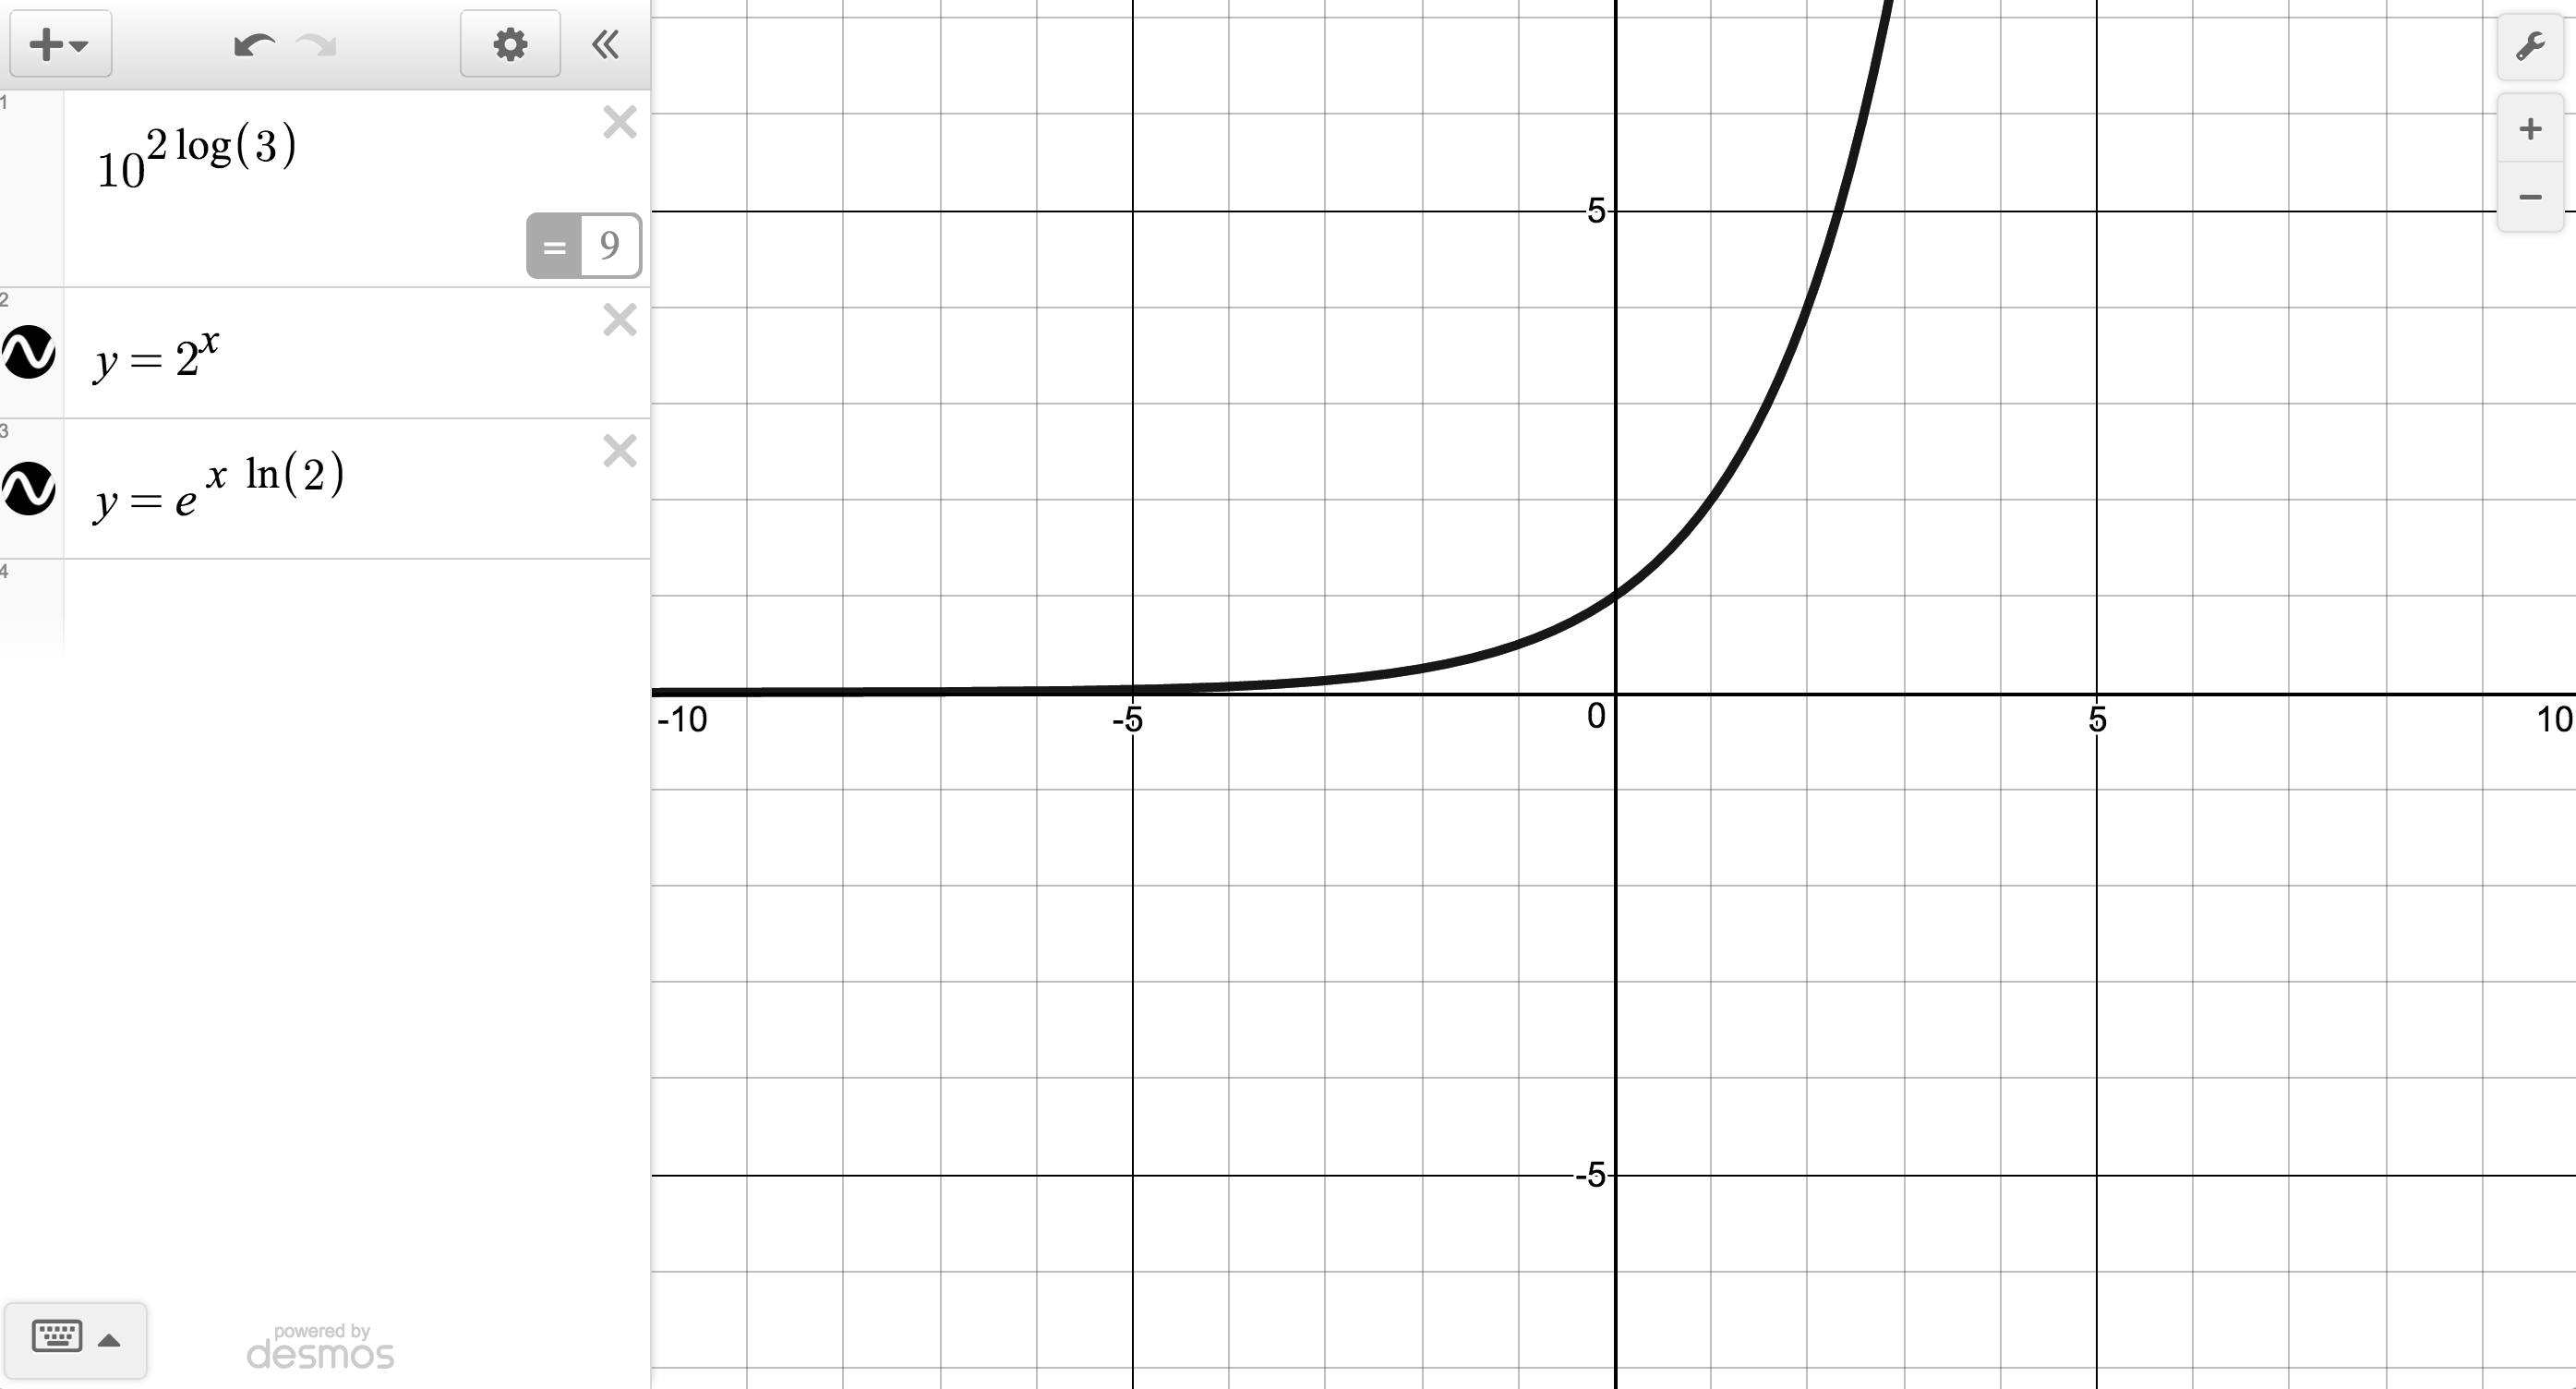
\includegraphics[width=4in]{./PropertiesofLogarithmsGraphics/LogProps01.jpg} 

\end{center}

\item  Applying the change of base with $a=4$ and $b=e$ leads us to write $\log_{4}(5) = \frac{\ln(5)}{\ln(4)}$.  Evaluating this gives the numerical approximation  $\frac{\ln(5)}{\ln(4)} \approx 1.16$. 

\smallskip

To check our answer we know that,  by definition, $\log_{4}(5)$ is the exponent we put on $4$ to get $5$, so a number a little larger than $1$ seems reasonable.

\smallskip

Taking this one step further, we use a graphing utility and find $4^{ \frac{\ln(5)}{\ln(4)}} = 5$, which means if  the machine  is lying to us about the first answer it gave us, at least it is being consistent.

\item  We write $\ln(x) = \log_{e}(x) = \frac{\log(x)}{\log(e)}$.  We graph both $f(x) = \ln(x)$ and $g(x) = \frac{\log(x)}{\log(e)}$ and find both graphs appear to be identical.

\begin{center}

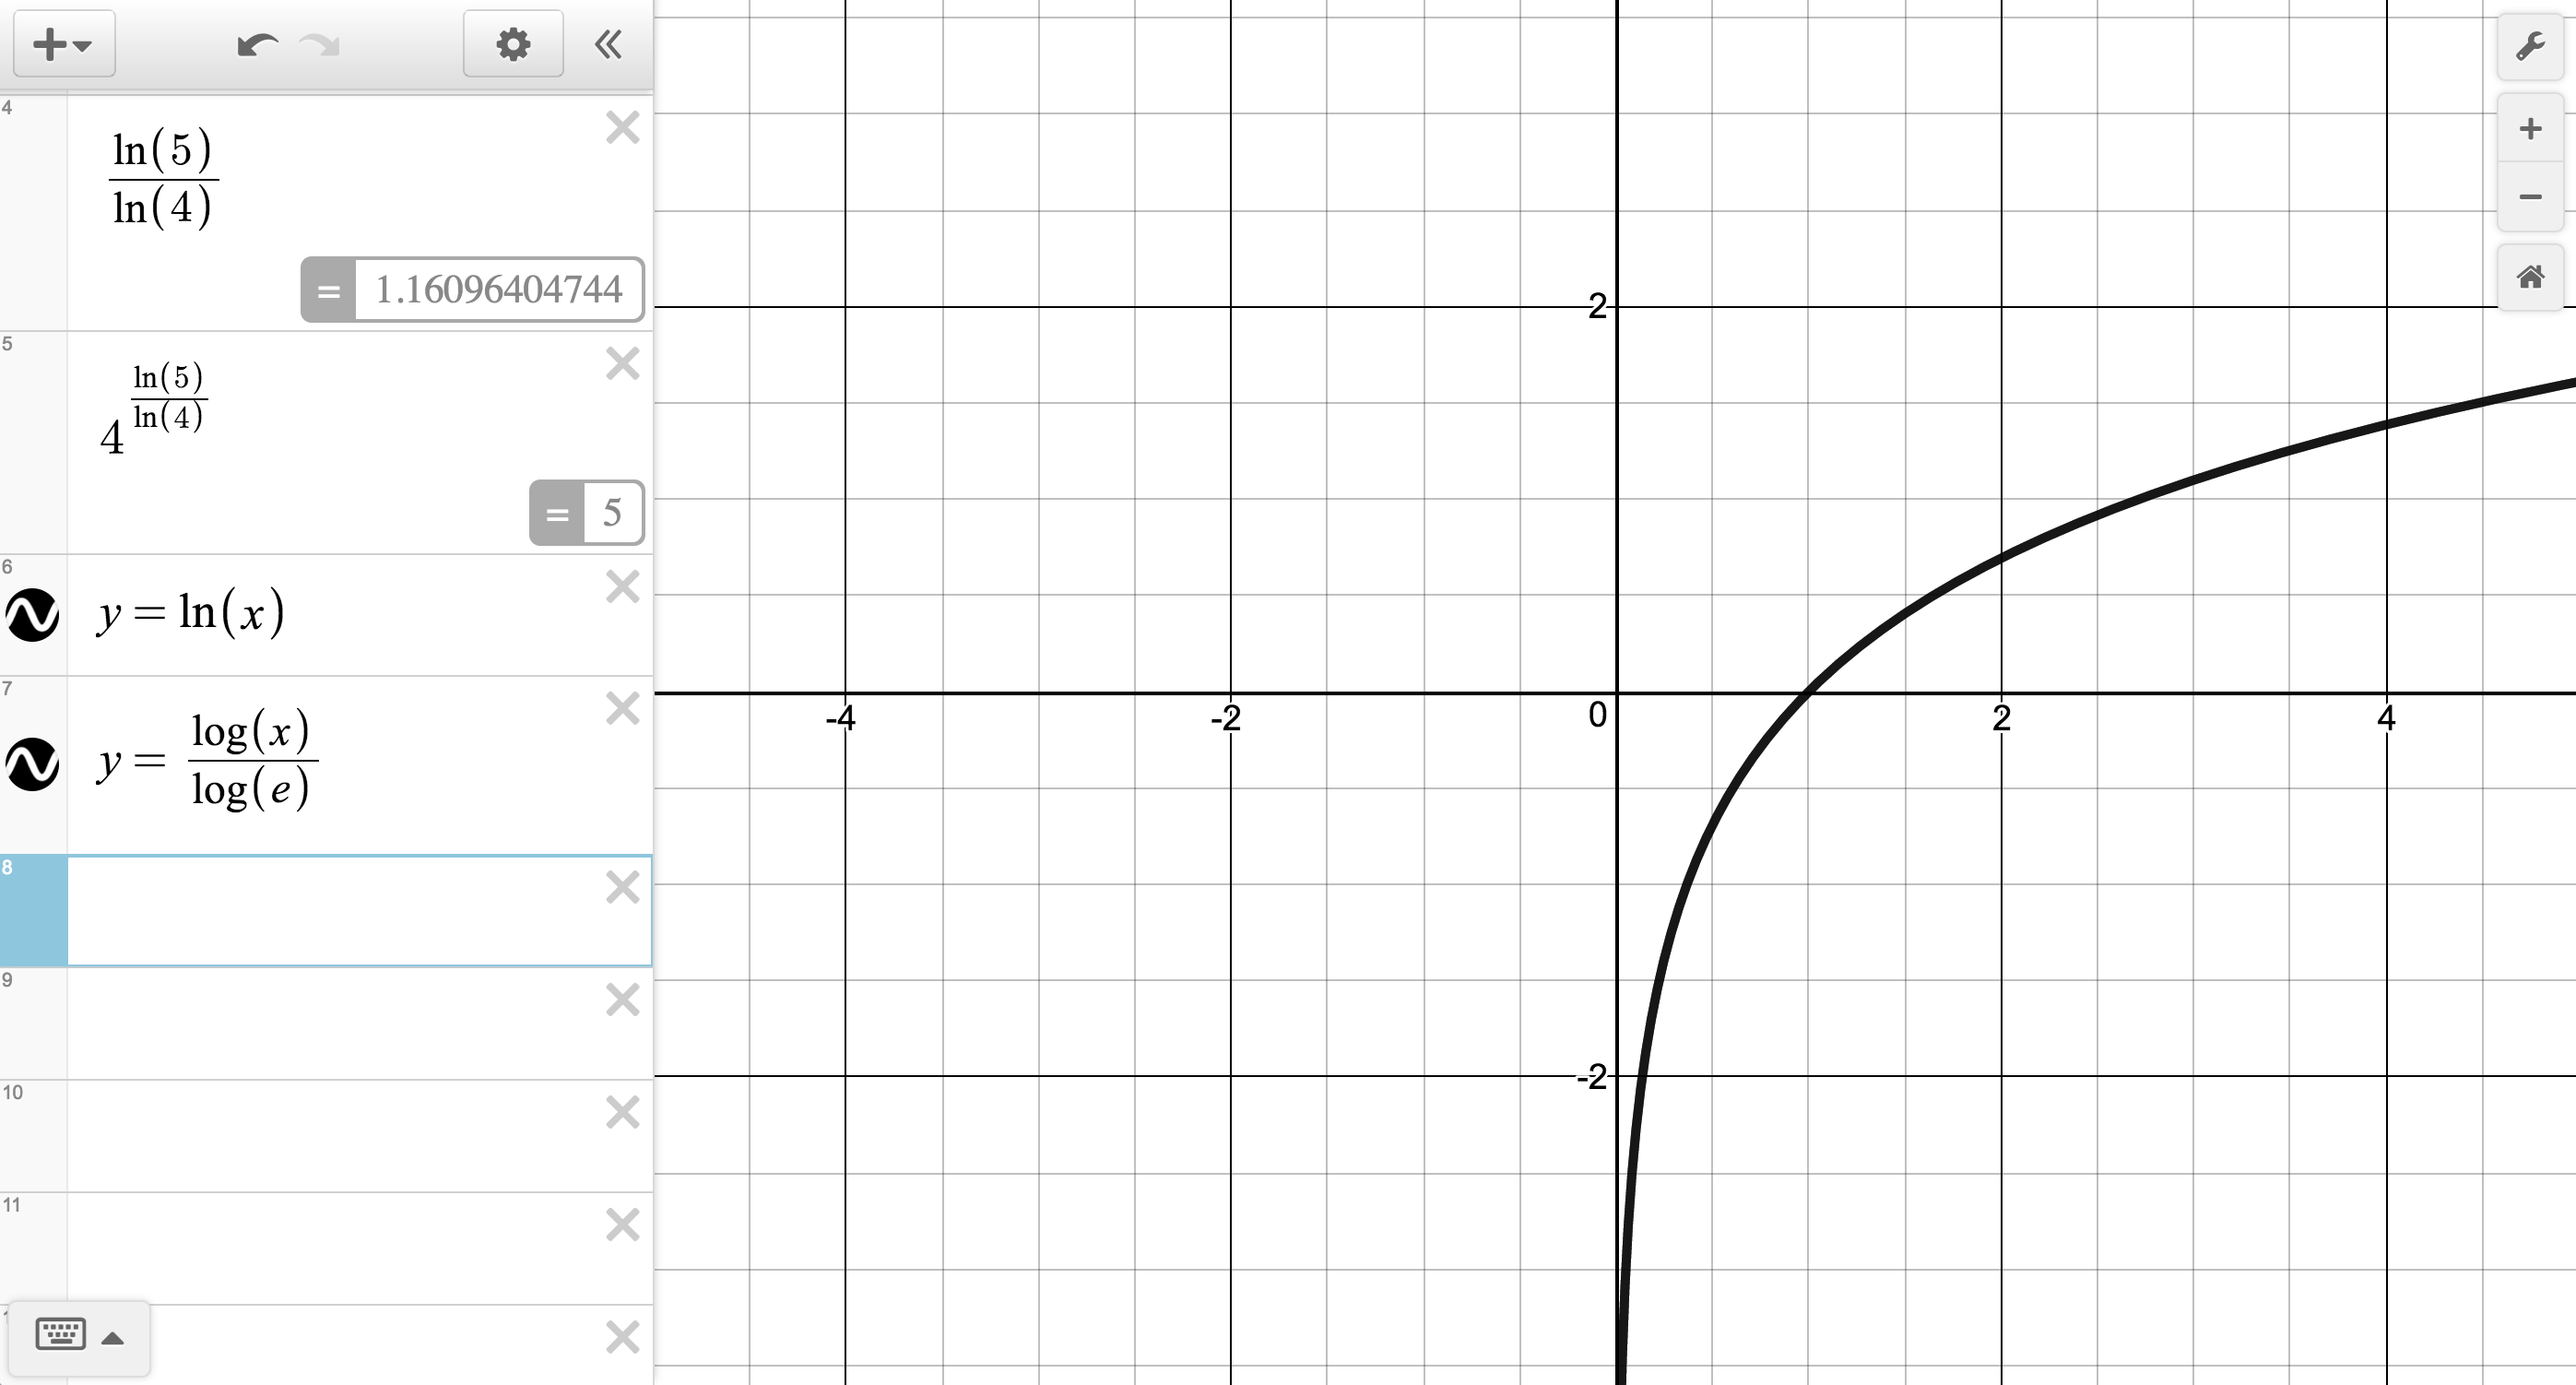
\includegraphics[width=4in]{./PropertiesofLogarithmsGraphics/LogProps02.jpg} 

\end{center}

\end{enumerate}

 \qed

\end{ex}

What Theorem \ref{changeofbase} really tells us is that all exponential and logarithmic functions are just scalings of one another.  Not only does this explain why their graphs have similar shapes, but it also tells us that we could do all of mathematics with a single base,  be it $10$, $0.42$, $\pi$, or $117$. 

\smallskip

As mentioned in Section \ref{ExponentialFunctions}, the `natural' base, base $e$, features prominently in mathematical applications\co{ as we'll see in Section \ref{ExpLogApplications}}.  Hence, we conclude this section by specifying  Theorem \ref{changeofbase} to this case.

\smallskip

\colorbox{ResultColor}{\bbm

\begin{thm}  \label{allbasee} \textbf{Conversion to the Natural Base:}  Suppose $b>0$, $b \neq 1$. Then

\begin{multicols}{2}

\begin{itemize}

\item $b^{x} = e^{x \ln(b)}$ for all real numbers $x$. \vphantom{$\log_{b}(x) = \dfrac{\ln(x)}{\ln(b)}$}

\item  $\log_{b}(x) = \dfrac{\ln(x)}{\ln(b)}$ for all real numbers $x > 0$.

\end{itemize}

\end{multicols}

\end{thm}

\smallskip

\ebm}



\newpage

\subsection{Exercises}

\label{ExercisesforPropertiesofLogarithms}

In Exercises \ref{expandlogfirst} - \ref{expandloglast}, expand the given logarithm and simplify.  Assume when necessary that all quantities represent positive real numbers.

\begin{multicols}{3}
\begin{enumerate}

\item $\ln(x^{3}y^{2})$ \vphantom{$\log_{2}\left(\dfrac{128}{x^{2} + 4}\right)$} \label{expandlogfirst}
\item $\log_{2}\left(\dfrac{128}{x^{2} + 4}\right)$
\item $\log_{5}\left(\dfrac{z}{25}\right)^{3}$ \vphantom{$\log_{2}\left(\dfrac{128}{x^{2} + 4}\right)$}

\setcounter{HW}{\value{enumi}}
\end{enumerate}
\end{multicols}

\begin{multicols}{3}
\begin{enumerate}
\setcounter{enumi}{\value{HW}}

\item $\log(1.23 \times 10^{37})$ \vphantom{$\ln\left(\dfrac{\sqrt{z}}{xy}\right)$}
\item $\ln\left(\dfrac{\sqrt{z}}{xy}\right)$
\item $\log_{5} \left(x^2 - 25 \right)$ \vphantom{$\ln\left(\dfrac{\sqrt{z}}{xy}\right)$}

\setcounter{HW}{\value{enumi}}
\end{enumerate}
\end{multicols}

\begin{multicols}{3}
\begin{enumerate}
\setcounter{enumi}{\value{HW}}

\item $\log_{\sqrt{2}} \left(4x^3\right)$
\item $\log_{\frac{1}{3}}(9x(y^{3} - 8))$
\item $\log\left(1000x^3y^5\right)$

\setcounter{HW}{\value{enumi}}
\end{enumerate}
\end{multicols}

\begin{multicols}{3}
\begin{enumerate}
\setcounter{enumi}{\value{HW}}

\item $\log_{3} \left(\dfrac{x^2}{81y^4}\right)$
\item $\ln\left(\sqrt[4]{\dfrac{xy}{ez}}\right)$
\item $\log_{6} \left(\dfrac{216}{x^3y}\right)^4$

\setcounter{HW}{\value{enumi}}
\end{enumerate}
\end{multicols}

\begin{multicols}{3}
\begin{enumerate}
\setcounter{enumi}{\value{HW}}

\item $\log\left(\dfrac{100x\sqrt{y}}{\sqrt[3]{10}}\right)$ \vphantom{$\log_{\frac{1}{2}}\left(\dfrac{4\sqrt[3]{x^2}}{y\sqrt{z}}\right)$}
\item $\log_{\frac{1}{2}}\left(\dfrac{4\sqrt[3]{x^2}}{y\sqrt{z}}\right)$
\item $\ln \left(\dfrac{\sqrt[3]{x}}{10 \sqrt{yz}}\right)$ \vphantom{$\log_{\frac{1}{2}}\left(\dfrac{4\sqrt[3]{x^2}}{y\sqrt{z}}\right)$} \label{expandloglast}

\setcounter{HW}{\value{enumi}}
\end{enumerate}
\end{multicols}

In Exercises \ref{combinelogfirst} - \ref{combineloglast}, use the properties of logarithms to write the expression as a single logarithm.

\begin{multicols}{2}
\begin{enumerate}
\setcounter{enumi}{\value{HW}}

\item $4\ln(x) + 2\ln(y)$ \label{combinelogfirst}
\item $\log_{2}(x) + \log_{2}(y) - \log_{2}(z)$

\setcounter{HW}{\value{enumi}}
\end{enumerate}
\end{multicols}

\begin{multicols}{2}
\begin{enumerate}
\setcounter{enumi}{\value{HW}}

\item $\log_{3}(x) - 2 \log_{3}(y)$
\item $\frac{1}{2}\log_{3}(x) - 2\log_{3}(y) - \log_{3}(z)$

\setcounter{HW}{\value{enumi}}
\end{enumerate}
\end{multicols}

\begin{multicols}{2}
\begin{enumerate}
\setcounter{enumi}{\value{HW}}
\item $2 \ln(x) -3 \ln(y) - 4\ln(z)$
\item $\log(x) - \frac{1}{3} \log(z) + \frac{1}{2} \log(y)$

\setcounter{HW}{\value{enumi}}
\end{enumerate}
\end{multicols}

\begin{multicols}{2}
\begin{enumerate}
\setcounter{enumi}{\value{HW}}

\item $-\frac{1}{3} \ln(x) - \frac{1}{3}\ln(y) + \frac{1}{3} \ln(z)$
\item $\log_{5}(x) - 3$

\setcounter{HW}{\value{enumi}}
\end{enumerate}
\end{multicols}

\begin{multicols}{2}
\begin{enumerate}
\setcounter{enumi}{\value{HW}}

\item $3 - \log(x)$
\item $\log_{7}(x) + \log_{7}(x - 3) - 2$

\setcounter{HW}{\value{enumi}}
\end{enumerate}
\end{multicols}

\begin{multicols}{2}
\begin{enumerate}
\setcounter{enumi}{\value{HW}}

\item $\ln(x) + \frac{1}{2}$ 
\item $\log_{2}(x) + \log_{4}(x)$ 

\setcounter{HW}{\value{enumi}}
\end{enumerate}
\end{multicols}

\begin{multicols}{2}
\begin{enumerate}
\setcounter{enumi}{\value{HW}}

\item $\log_{2}(x) + \log_{4}(x-1)$
\item $\log_{2}(x) + \log_{\frac{1}{2}}(x - 1)$ \label{combineloglast}

\setcounter{HW}{\value{enumi}}
\end{enumerate}
\end{multicols}


In Exercises \ref{changeofbasefirst} - \ref{changeofbaselast}, use the appropriate change of base formula to convert the given expression to an expression with the indicated base. 

\begin{multicols}{2}
\begin{enumerate}
\setcounter{enumi}{\value{HW}}

\item $7^{x - 1}$ to base $e$ \label{changeofbasefirst}
\item $\log_{3}(x + 2)$ to base 10

\setcounter{HW}{\value{enumi}}
\end{enumerate}
\end{multicols}

\begin{multicols}{2}
\begin{enumerate}
\setcounter{enumi}{\value{HW}}

\item $\left(\dfrac{2}{3}\right)^{x}$ to base $e$
\item $\log(x^{2} + 1)$ to base $e$ \vphantom{$\left(\dfrac{2}{3}\right)^{x}$}\label{changeofbaselast}

\setcounter{HW}{\value{enumi}}
\end{enumerate}
\end{multicols}

\newpage

In Exercises \ref{changeofbaseapproxfirst} - \ref{changeofbaseapproxlast}, use the appropriate change of base formula to approximate the logarithm.

\begin{multicols}{3}
\begin{enumerate}
\setcounter{enumi}{\value{HW}}

\item $\log_{3}(12)$ \label{changeofbaseapproxfirst}
\item $\log_{5}(80)$
\item $\log_{6}(72)$

\setcounter{HW}{\value{enumi}}
\end{enumerate}
\end{multicols}

\begin{multicols}{3}
\begin{enumerate}
\setcounter{enumi}{\value{HW}}

\item $\log_{4}\left(\dfrac{1}{10}\right)$
\item $\log_{\frac{3}{5}}(1000)$ \vphantom{$\log_{4}\left(\dfrac{1}{10}\right)$}
\item $\log_{\frac{2}{3}}(50)$ \vphantom{$\log_{4}\left(\dfrac{1}{10}\right)$} \label{changeofbaseapproxlast}

\setcounter{HW}{\value{enumi}}
\end{enumerate}
\end{multicols}

\begin{enumerate}
\setcounter{enumi}{\value{HW}}

\item \label{morethanoneforlogexercise} In Example \ref{intrologex} number \ref{findformulaforlogexample} in Section \ref{LogarithmicFunctions}, we obtained the solution  $F(x) = \log_{2}(-x+4)-3$ as one formula for the given graph by making a simplifying assumption that $b = -1$.  This exercises explores if there are any other solutions for different choices of $b$.

\begin{enumerate}

\item  Show  $G(x) =\log_{2}(-2x+8) - 4$ also fits the data for the given graph.

\item  Use properties of logarithms to show $G(x) = \log_{2}(-2x+8) -4  = \log_{2}(-x+4)-3 = F(x)$.

\item  With help from your classmates, find solutions to Example \ref{intrologex} number \ref{findformulaforlogexample} in Section \ref{LogarithmicFunctions} by assuming $b = -4$ and $b = -8$.  In each case, use properties of logarithms to show the solutions reduce to $F(x) = \log_{2}(-x+4)-3$.

\item  Using properties of logarithms and the fact that the range of $\log_{2}(x)$ is all real numbers, show that any function of the form $f(x) = a \log_{2}(bx-h) + k$ where $a \neq 0$ can be rewritten as: 

\[ f(x) = a \left( \log_{2}(bx-h) +  \frac{k}{a}\right) = a ( \log_{2}(bx -h) + \log_{2}(p)) = a \log_{2}(p(bx-h)) = a \log_{2}(pbx - ph),\]

where $\frac{k}{a} = \log_{2}(p)$ for some positive real number $p$. Relabeling, we get every function of the form $f(x) = a \log_{2}(bx-h) + k$ with four parameters ($a$, $b$, $h$, and $k$) can be rewritten as $f(x) = a \log_{2}(Bx - H)$, a formula with just three parameters: $a$, $B$, and $H$.

\smallskip

Show \textit{every} solution to Example \ref{intrologex} number \ref{findformulaforlogexample} in Section \ref{LogarithmicFunctions} can be written in the form  $f(x) = \log_{2}\left( -\frac{1}{8}  x + \frac{1}{2} \right)$ and that, in particular,  $F(x) = \log_{2}(-x+4) -3 = \log_{2}\left( -\frac{1}{8}  x + \frac{1}{2} \right) = f(x)$.  Hence, there is really just one solution to Example \ref{intrologex} number \ref{findformulaforlogexample} in Section \ref{LogarithmicFunctions}.

\end{enumerate}   

\item \label{HendersonHasselbalch} \index{Henderson-Hasselbalch Equation} The Henderson-Hasselbalch Equation:  Suppose $HA$ represents a weak acid. Then we have a reversible chemical reaction 
\[HA \rightleftharpoons H^{+} + A^{-}.\]  
The acid disassociation constant, $K_{a}$, is given by 
\[K_{a} = \frac{[H^{+}][A^{-}]}{[HA]} = [H^{+}]\frac{[A^{-}]}{[HA]},\]
where the square brackets denote the concentrations just as they did in Exercise \ref{pHexercise} in Section \ref{LogarithmicFunctions}.  The symbol p$K_{a}$ is defined similarly to pH in that p$K_{a} = -\log(K_{a})$.  Using the definition of pH from Exercise \ref{pHexercise} and the properties of logarithms, derive the Henderson-Hasselbalch Equation:

\[\mbox{pH} = \mbox{p}K_{a} + \log\dfrac{[A^{-}]}{[HA]}\]

\item Compare and contrast the graphs of $y = \ln(x^{2})$ and $y = 2\ln(x)$.

\item Prove the Quotient Rule and Power Rule for Logarithms.

\item Give numerical examples to show that, in general,

\begin{multicols}{2}
\begin{enumerate}

\item $\log_{b}(x + y) \neq \log_{b}(x) + \log_{b}(y)$
\item $\log_{b}(x - y) \neq \log_{b}(x) - \log_{b}(y)$
\setcounter{HWindent}{\value{enumii}}
\end{enumerate}
\end{multicols}

\begin{enumerate}
\setcounter{enumii}{\value{HWindent}}

\item $\log_{b}\left(\dfrac{x}{y}\right) \neq \dfrac{\log_{b}(x)}{\log_{b}(y)}$

\end{enumerate}

\item Research the history of logarithms including the origin of the word `logarithm' itself.  Why is the abbreviation of natural log `ln' and not `nl'?

\item There is a scene in the movie `Apollo 13' in which several people at Mission Control use slide rules to verify a computation.  Was that scene accurate?  Look for other pop culture references to logarithms and slide rules.


\setcounter{HW}{\value{enumi}}
\end{enumerate}


\newpage

\subsection{Answers}


\begin{multicols}{2}
\begin{enumerate}

\item $3\ln(x) + 2\ln(y)$
\item $7 - \log_{2}(x^{2} + 4)$

\setcounter{HW}{\value{enumi}}
\end{enumerate}
\end{multicols}

\begin{multicols}{2}
\begin{enumerate}
\setcounter{enumi}{\value{HW}}


\item $3\log_{5}(z) - 6$
\item $\log(1.23) + 37$

\setcounter{HW}{\value{enumi}}
\end{enumerate}
\end{multicols}

\begin{multicols}{2}
\begin{enumerate}
\setcounter{enumi}{\value{HW}}

\item $\frac{1}{2}\ln(z) - \ln(x) - \ln(y)$
\item  $\log_{5}(x-5) + \log_{5}(x+5)$

\setcounter{HW}{\value{enumi}}
\end{enumerate}
\end{multicols}

\begin{multicols}{2}
\begin{enumerate}
\setcounter{enumi}{\value{HW}}

\item  $3\log_{\sqrt{2}}(x) + 4$
\item \small$-2 + \log_{\frac{1}{3}}(x) + \log_{\frac{1}{3}}(y - 2) + \log_{\frac{1}{3}}(y^{2} + 2y + 4)$\normalsize

\setcounter{HW}{\value{enumi}}
\end{enumerate}
\end{multicols}

\begin{multicols}{2}
\begin{enumerate}
\setcounter{enumi}{\value{HW}}

\item $3 + 3\log(x) + 5 \log(y)$
\item $2\log_{3}(x) - 4 - 4\log_{3}(y)$

\setcounter{HW}{\value{enumi}}
\end{enumerate}
\end{multicols}

\begin{multicols}{2}
\begin{enumerate}
\setcounter{enumi}{\value{HW}}

\item $\frac{1}{4} \ln(x) + \frac{1}{4} \ln(y) - \frac{1}{4} - \frac{1}{4} \ln(z)$
\item $12-12\log_{6}(x) - 4\log_{6}(y)$

\setcounter{HW}{\value{enumi}}
\end{enumerate}
\end{multicols}

\begin{multicols}{2}
\begin{enumerate}
\setcounter{enumi}{\value{HW}}

\item $\frac{5}{3}+\log(x)+\frac{1}{2}\log(y)$
\item $-2+\frac{2}{3}\log_{\frac{1}{2}}(x)-\log_{\frac{1}{2}}(y)-\frac{1}{2}\log_{\frac{1}{2}}(z)$

\setcounter{HW}{\value{enumi}}
\end{enumerate}
\end{multicols}

\begin{multicols}{2}
\begin{enumerate}
\setcounter{enumi}{\value{HW}}

\item $\frac{1}{3} \ln(x) - \ln(10) - \frac{1}{2}\ln(y)-\frac{1}{2}\ln(z)$
\item $\ln(x^{4}y^{2})$
\setcounter{HW}{\value{enumi}}
\end{enumerate}
\end{multicols}

\begin{multicols}{3}
\begin{enumerate}
\setcounter{enumi}{\value{HW}}

\item $\log_{2}\left(\frac{xy}{z}\right)$
\item $\log_{3} \left( \frac{x}{y^2} \right)$
\item $\log_{3}\left(\frac{\sqrt{x}}{y^{2}z}\right)$

\setcounter{HW}{\value{enumi}}
\end{enumerate}
\end{multicols}

\begin{multicols}{3}
\begin{enumerate}
\setcounter{enumi}{\value{HW}}


\item $\ln\left( \frac{x^2}{y^3z^4} \right)$
\item $\log\left(\frac{x \sqrt{y}}{\sqrt[3]{z}}  \right)$
\item $\ln\left(\sqrt[3]{\frac{z}{xy}}   \right)$

\setcounter{HW}{\value{enumi}}
\end{enumerate}
\end{multicols}

\begin{multicols}{3}
\begin{enumerate}
\setcounter{enumi}{\value{HW}}

\item $\log_{5}\left(\frac{x}{125}\right)$
\item $\log\left(\frac{1000}{x}\right)$
\item $\log_{7}\left(\frac{x(x - 3)}{49}\right)$

\setcounter{HW}{\value{enumi}}
\end{enumerate}
\end{multicols}

\begin{multicols}{3}
\begin{enumerate}
\setcounter{enumi}{\value{HW}}

\item $\ln \left(x \sqrt{e} \right)$
\item $\log_{2}\left(x^{3/2}\right)$
\item $\log_{2}\left(x \sqrt{x-1}\right)$


\setcounter{HW}{\value{enumi}}
\end{enumerate}
\end{multicols}


\begin{multicols}{3}
\begin{enumerate}
\setcounter{enumi}{\value{HW}}
\item $\vphantom{\frac{\log(x + 2)}{\log(3)}}\log_{2}\left(\frac{x}{x - 1}\right)$ 
\item $\vphantom{\frac{\log(x + 2)}{\log(3)}}7^{x - 1} = e^{(x - 1)\ln(7)}$
\item $\log_{3}(x + 2) = \frac{\log(x + 2)}{\log(3)}$


\setcounter{HW}{\value{enumi}}
\end{enumerate}
\end{multicols}


\begin{multicols}{2}
\begin{enumerate}
\setcounter{enumi}{\value{HW}}

\item $\left(\frac{2}{3}\right)^{x} = e^{x\ln(\frac{2}{3})}$
\item $\log(x^{2} + 1) = \frac{\ln(x^{2} + 1)}{\ln(10)}$

\setcounter{HW}{\value{enumi}}
\end{enumerate}
\end{multicols}

\begin{multicols}{2}
\begin{enumerate}
\setcounter{enumi}{\value{HW}}

\item $\log_{3}(12) \approx 2.26186$
\item $\log_{5}(80) \approx 2.72271$

\setcounter{HW}{\value{enumi}}
\end{enumerate}
\end{multicols}

\begin{multicols}{2}
\begin{enumerate}
\setcounter{enumi}{\value{HW}}

\item $\log_{6}(72) \approx 2.38685$
\item $\log_{4}\left(\frac{1}{10}\right) \approx -1.66096$

\setcounter{HW}{\value{enumi}}
\end{enumerate}
\end{multicols}

\begin{multicols}{2}
\begin{enumerate}
\setcounter{enumi}{\value{HW}}
\item $\log_{\frac{3}{5}}(1000) \approx -13.52273$
\item $\log_{\frac{2}{3}}(50) \approx -9.64824$

\setcounter{HW}{\value{enumi}}
\end{enumerate}
\end{multicols}


\closegraphsfile
